\documentclass[a4paper,french,bookmarks]{article}
\usepackage{./Structure/4PE18TEXTB}

\begin{document}
\stylize{Informatique}{Devoir Maison 1 : Enveloppes convexes dans le plan}

\textbf{Important :} les fichiers mentionnés dans ce sujet sont disponibles sur la page web du cours. Ce sujet est inspiré de l’épreuve X/ENS info B, adaptée pour le langage C par Marc de Falco.\\

Ce sujet a pour objectif de calculer des enveloppes convexes de nuages de points dans le plan affine, ungrand classique en géométrie algorithmique. On dit qu’un ensemble $C \subset \bdR^2$ est convexe si et seulement si pour toute paire de points $(p, q) \in C^2$, le segment de droite $[p, q]$ est inclus dans $C$. L’enveloppe convexe d’un ensemble $P \subset \bdR^2$, notée $Conv(P)$, est le plus petit convexe contenant $P$. Dans le cas où $P$ est un ensemble fini (appelé nuage de points), le bord de $Conv(P)$ est un polygone convexe dont les sommets appartiennent à $P$, comme illustré dans la figure \ref{fig:fig1}.

\begin{figure}[!ht]
    \centering
    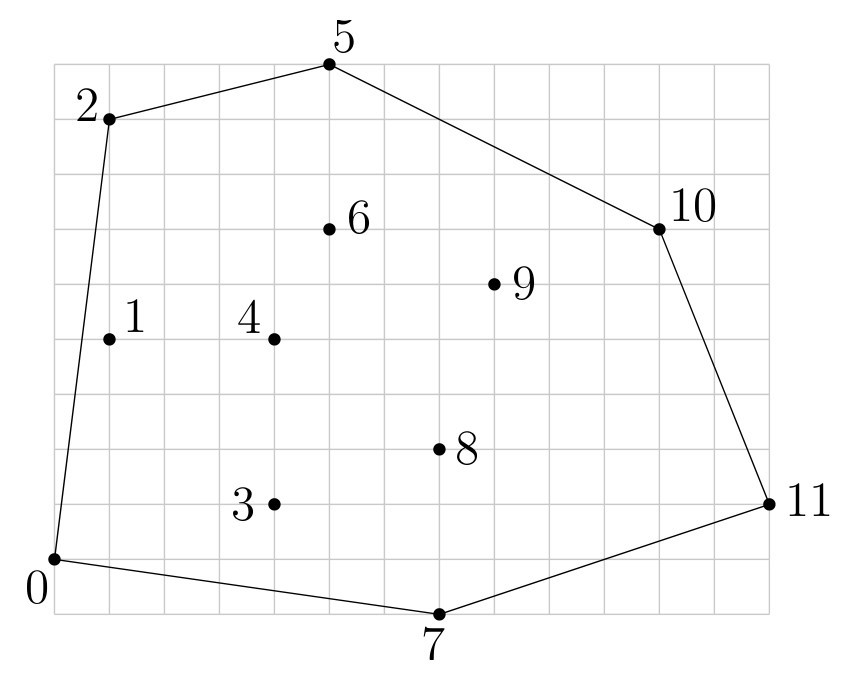
\includegraphics[width=0.3\textwidth]{dm1/figure1.jpg}
    \caption{Un nuage de points, numérotés de 0 à 11, et le bord de son enveloppe convexe.}
    \label{fig:fig1}
\end{figure}

Le calcul de l’enveloppe convexe d’un nuage de points est un problème fondamental en informatique, qui trouve des applications dans de nombreux domaines comme :
\begin{enumerate}
    \item[\bullet] la robotique, par exemple pour l’accélération de la détection de collisions dans le cadre de la planification de trajectoire ;
    \item[\bullet] le traitement d’images et la vision, par exemple pour la détection d’objets convexes (comme des plaques minéralogiques de voiture) dans des scènes 2D ;
    \item[\bullet] l’informatique graphique, par exemple pour l’accélération du rendu de scènes 3D par lancer de rayons ;
    \item[\bullet] la théorie des jeux, par exemple pour déterminer l’existence d’équilibres de Nash ;
    \item[\bullet] la vérification formelle, par exemple pour déterminer si une variable risque de dépasser sa capacité de stockage ou d’atteindre un ensemble de valeurs interdites lors de l’exécution d’une boucle dans un programme, et bien d’autres encore.
\end{enumerate}
Dans ce sujet nous allons écrire deux algorithmes de calcul du bord de l’enveloppe convexe d’un nuage de points $P$ dans le plan affine. Le premier, dit algorithme du \textbf{paquet cadeau}, consiste à envelopper le nuage de points $P$ progressivement en faisant pivoter une droite tout autour. Le deuxième, dit de \textbf{balayage}, consiste à balayer le plan horizontalement avec une droite verticale, tout en maintenant au fur et à mesure l’enveloppe convexe de la partie du nuage située à gauche de cette droite verticale. Les deux algorithmes sont illustrés respectivement dans les figures 3 et 4.\\

Le temps d’exécution du premier algorithme est majoré par une constante fois $nm$, celui du deuxième par une constante fois $n \log n$, où $n$ désigne le nombre total de points de $P$ et $m$ le nombre de points de $P$ appartenant au bord de $Conv(P)$.
Rappelons que le temps d’exécution d’un programme $A$ (fonction ou procédure) est le nombre d’opérations élémentaires (comparaisons, additions, soustractions, multiplications, divisions, affectations, etc.) nécessaires à l’exécution de $A$. Sauf mention contraire dans l’énoncé du
sujet, le candidat n’aura pas à justifier des temps de calcul de ses programmes. Toutefois, il devra veiller à ce que ces derniers ne dépassent pas les bornes prescrites.\\

On va représenter les points par des éléments du type \verb|point| : 

\begin{code}{c}{point.h}
struct point {
    int x;
    int y;
};
typedef struct point point;
\end{code}

Dans toute la suite on supposera que le nuage de points $P$ est de taille $n \geq 3$ et en position générale, c’est-à-dire qu’il ne contient pas 3 points distincts alignés. Ces hypothèses vont permettre de simplifier les calculs en ignorant les cas pathologiques, comme par exemple la présence de 3 points alignés sur le bord de l’enveloppe convexe. Nos programmes prendront en entrée un nuage de points $P$ dont les coordonnées sont stockées dans un tableau \verb|tab| de \verb|point|, comme dans l’exemple ci-dessous qui contient les coordonnées du nuage de points de la figure 1 :

\begin{code}{c}{figure1.c}
point tab[] = {
        { 0, 0 }, { 1, 4 }, { 1, 8 }, { 4, 1 }, { 4, 4 }, { 5, 9 },
        { 5, 6 }, { 7, -1 }, { 7, 2 }, { 8, 5 }, { 11, 6 }, { 13, 1 }
}; // initialisation directe des struct comme pour les tableaux
\end{code}

Précisons que les coordonnées, supposées entières, sont données dans une base orthonormée du plan, orientée dans le sens direct.

\subsection*{A - Préliminaires}

\begin{enumerate}
    \item Écrire une fonction \verb|int plus_bas(point *tab, int n);| qui prend en paramètre le tableau \verb|tab| de $n$ points et qui renvoie l’indice $j$ du point le plus bas (c’est-à-dire de plus petite ordonnée) parmi les points du nuage $P$. En cas d’égalité, votre fonction devra renvoyer l’indice du point de plus petite abscisse parmi les points les plus bas.
    
    \begin{code}{c}{main.c}
int plus_bas(point *tab, int n) {
    int pos = 0;
    for (int i = pos; i < n; i++) {
        if (tab[i].y < tab[pos].y ||
                (tab[i].y == tab[pos].y && tab[i].x <= tab[pos].x)) {
            pos = i;
        }
    }
    return pos;
}
    \end{code}

    \item Prouver la correction de cette fonction. Sur le tableau exemple précédent, le résultat doit être l’indice 6.
    
    \boxans{
        Soit $P$ un nuage de $n$ points. On définit la relation d'ordre $\preccurlyeq$ par :
        \[ \forall (p, p') \in P, \quad p \preccurlyeq p' \iff p.y < p'.y \qquad \mathrm{OU} \qquad (p.y = p'.y \quad \mathrm{ET} \quad p.x \leq p'.x)\]
        On note $P[i]$ le point dans $P$ d'indice $i \in \llbracket0;n-1\rrbracket$. Pour $i \in \llbracket0;n-1\rrbracket$, on pose l'invariant de boucle suivant :
        \[ C(i) : \forall k \in \llbracket0;i\rrbracket, \qquad P[pos] \preccurlyeq P[k]\]
        
        $C(0)$ est vrai car initialement $\texttt{pos} := 0$ et $\preccurlyeq$ est réflexive donc $P[\texttt{pos}] \preccurlyeq P[0]$.
        
        Soit $i \in \llbracket0;n-1\rrbracket$ tel que $C(i)$ est vrai.
        
        Si $P[\texttt{pos}].y < P[i+1].y$, alors $P[\texttt{pos}] \preccurlyeq P[i+1]$, donc $C(i+1)$ est vrai.
        
        Si $P[\texttt{pos}].y = P[i+1].y$ et $P[\texttt{pos}].x \leq P[i+1].x$, de même.
        
        Sinon, $P[i+1] \preccurlyeq P[\texttt{pos}]$, donc $\forall k \in \llbracket0;i+1\rrbracket, \qquad P[i+1] \preccurlyeq P[k]$. 
        
        On redéfinit alors $\texttt{pos} := i+1$, donc $C(i+1)$ est vrai. Donc $C(i) \implies C(i+1)$.
        
        Par récurrence, on a montré que $\forall k \in \llbracket0;n-1\rrbracket, \qquad P[\texttt{pos}] \preccurlyeq P[k]$, donc $\forall p \in P, \quad P[\texttt{pos}] \preccurlyeq p$.
        Puisqu'elle renvoie le contenu variable $\texttt{pos} = \min_\preccurlyeq P$, \boxsol{on a montré la correction de cette fonction}.
    }
    
    Dans la suite nous aurons besoin d’effectuer un seul type de test géométrique : celui de l’orientation.
\end{enumerate}

\textbf{Définition 1} \begin{itshape}
Étant donnés trois points $p_i$, $p_j$, $p_k$ du nuage $P$, distincts ou non, le test d’orientation renvoie $+1$ si la séquence $(p_i, p_j , p_k)$ est orientée positivement, $−1$ si elle est orientée négativement, et $0$ si les trois points sont alignés (c’est-à-dire si deux au moins sont égaux, d’après l’hypothèse de position générale).
\end{itshape}

Pour déterminer l’orientation de $(p_i, p_j , p_k)$, il suffit de calculer l’aire signée du triangle, comme illustré sur la figure \ref{fig:fig2}.

Cette aire vaut :
\[ \dfrac{1}{2}\left((y_k-y_i)(x_j-x_i) - (x_k-x_i)(y_j-y_i)\right)\]
où $p_a$ a pour coordonnées $(x_a, y_a)$. \textbf{Comme on travaille avec des entiers, on évitera de faire la division par 2 qui peut aboutir à 0 et ne préserve pas le signe strict.}

\begin{figure}[!ht]
    \centering
    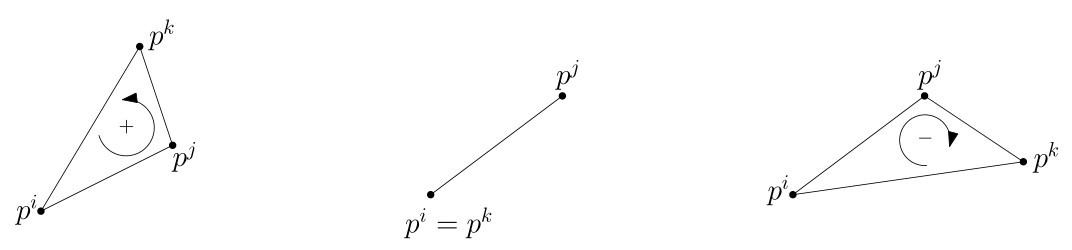
\includegraphics[width=0.6\textwidth]{dm1/figure2.jpg}
    \caption{Test d’orientation sur la séquence $(p_i, p_j , p_k)$ : positif à gauche, nul au centre, négatif à droite.}
    \label{fig:fig2}
\end{figure}

\begin{enumerate}[resume]
    \item Sur le tableau exemple précédent, donner le résultat du test d’orientation pour les choix d’indices suivants :
    
    1. $i = 0$, $j = 3$, $k = 4$, \qquad\qquad 2. $i = 8$, $j = 9$, $k = 10$
    
    \boxans{
        Pour $i = 0$, $j = 3$, $k = 4$, \boxsol{le test renvoie +1}. Pour $i = 8$, $j = 9$, $k = 10$, \boxsol{le test renvoie -1}.
    }
    
    \item Écrire une fonction \verb|int orient(point *tab, int i, int j, int k);| qui prend en paramètres le tableau \verb|tab| et trois indices, potentiellement égaux, et qui renvoie le résultat (−1, 0 ou +1) du test d’orientation sur la séquence $(p_i, p_j , p_k)$ de points de $P$.
    
    \begin{code}{c}{main.c}
int orient(point *tab, int i, int j, int k) {
    int area = ((tab[k].y - tab[i].y)*(tab[j].x - tab[i].x) - 
            (tab[k].x - tab[i].x)*(tab[j].y - tab[i].y));
    return area > 0 ? 1 : (area < 0 ? -1 : 0);
}
    \end{code}
\end{enumerate}

\subsection*{B - Algorithme du paquet cadeau}

Cet algorithme a été proposé par R. Jarvis en 1973. Il consiste à envelopper peu à peu le nuage de points $P$ dans une sorte de paquet cadeau, qui à la fin du processus est exactement le bord de $Conv(P)$. On commence par insérer le point de plus petite ordonnée (celui d’indice 7 dans l’exemple de la figure 1) dans le paquet cadeau, puis à chaque étape de la procédure on sélectionne le prochain point du nuage $P$ à insérer. 

La procédure de sélection fonctionne comme suit. Soit $p_i$ le dernier point inséré dans le paquet cadeau à cet instant. Par exemple, $i = 10$ dans l’exemple de la figure \ref{fig:fig3}.

\begin{figure}[!ht]
    \centering
    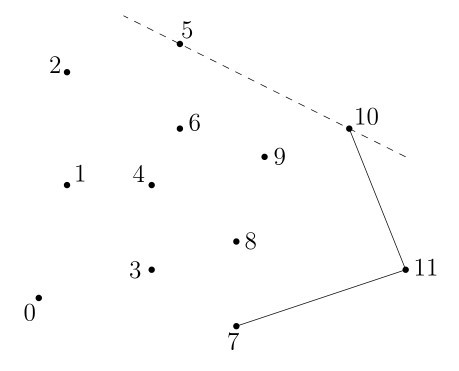
\includegraphics[width=0.3\textwidth]{dm1/figure3.jpg}
    \caption{Mise à jour du paquet cadeau après insertion du point $p_0$.}
    \label{fig:fig3}
\end{figure}

Considérons la relation binaire $\preccurlyeq$ définie sur l’ensemble $P\backslash\{p_i\}$ par :
\[ p_j \preccurlyeq p_k \iff \verb|orient(tab, i, j, k)| \leq 0\]

\begin{enumerate}[resume]
    \item Justifier brièvement le fait que $\preccurlyeq$ est une relation d'ordre total sur l'ensemble  $P\backslash\{p_i\}$.
    
    Ainsi, le prochain point à insérer (le point d’indice 5 dans la figure 3) est l’élément maximum pour la relation d’ordre $\preccurlyeq$. Il peut se calculer en temps linéaire (c’est-à-dire majoré par une constante fois n) par une simple itération sur les points de $P\backslash\{p_i\}$.
    
    \boxans{
        On a $\texttt{orient(tab, i, j, j)} = 0$ donc $\texttt{orient(tab, i, j, j)} \leq 0$ donc $p_j \preccurlyeq p_j$ donc $\preccurlyeq$ est réflexive.
        
        Si $\left\lbrace\begin{array}{lc}
            p_j &\preccurlyeq p_k \\
            p_k &\preccurlyeq p_j
        \end{array}\right.$ alors $\left\lbrace\begin{array}{lc}
            \texttt{orient(tab, i, j, k)} &\leq 0 \\
            \texttt{orient(tab, i, k, j)} &\leq 0
        \end{array}\right.$ alors $\left\lbrace\begin{array}{lc}
            \texttt{orient(tab, i, j, k)} &\leq 0 \\
            \texttt{orient(tab, i, j, k)} &\geq 0
        \end{array}\right.$ alors $\texttt{orient(tab, i, j, k)} = 0$ alors $p_j = p_k$, donc $\preccurlyeq$ est antisymétrique.
        }
    \boxans{
        Si $\left\lbrace\begin{array}{lc}
            p_j &\preccurlyeq p_k \\
            p_k &\preccurlyeq p_l
        \end{array}\right.$ alors $\left\lbrace\begin{array}{lc}
            \texttt{orient(tab, i, j, k)} &\leq 0 \\
            \texttt{orient(tab, i, k, l)} &\leq 0
        \end{array}\right.$ alors $\left\lbrace\begin{array}{lc}
            \widehat{p_jp_ip_k} &\leq 0 \\
            \widehat{p_kp_ip_l} &\leq 0 
        \end{array}\right.$ alors $\widehat{p_jp_ip_l} \leq 0$ alors $\texttt{orient(tab, i, j, l)} \leq 0$ alors $ p_j \preccurlyeq p_l$ donc $\preccurlyeq$ est transitive.
        
        La relation binaire $\preccurlyeq$ est réfléxive, antisymétrique et transtitive donc c'est une relation d'ordre.
        
        Par ailleurs, $j \not\preccurlyeq k \implies \texttt{orient(tab, i, j, k)} > 0 \implies \texttt{orient(tab, i, k, j)} < 0 \implies k \preccurlyeq j$ donc \boxsol{$\preccurlyeq$ est une relation d'ordre totale}.
    }
    
    \item Écrire une fonction \verb|int prochain_point(point *tab, int n, int i);| qui prend en paramètre le tableau \verb|tab| de $n$ points ainsi que l’indice $i$ du point inséré en dernier dans le paquet cadeau, et qui renvoie l’indice du prochain point à insérer selon cette procédure. Le temps d’exécution de votre fonction doit être majoré par une constante fois $n$, pour tous $n$ et $i$. La constante doit être indépendante de $n$ et $i$, et on ne demande pas de la préciser.
    
    \begin{code}{c}{main.c}
int prochain_point(point *tab, int n, int i) {
    int pos = 0 + i==0;
    for (int k = pos; k < n; k+=1)
        if (k !=i && orient(tab, i, pos, k) < 0) pos = k;
    return pos;
}
    \end{code}
    
    \item Décrire à la main le déroulement de la fonction \verb|prochain_point| sur l’exemple de la figure \ref{fig:fig3}. Plus précisément, indiquer la séquence des points de $P\backslash\{p_{10}\}$ considérés et la valeur de l’indice du maximum à chaque itération.
    
    \boxans{
        La fonction $\texttt{prochain\_point}$ utilise une variable locale $\texttt{pos} := 0$ qui représente l'indice du maximum selon $\preccurlyeq$ dans $P\backslash\{p_{10}\}$.
        A chaque itération, la fonction compare le $k$-ième élément de $P\backslash\{p_{10}\}$ avec le maximum des $k-1$-ièmes précédents éléments : s'il est plus grand, alors on redéfinit $\texttt{pos} := k$.
        
        On a alors pour les indices $k$ les maximums respectifs $\texttt{pos}$ suivants :\\
        
        \renewcommand\arraystretch{1.5}
        \centering\begin{tabular}{|p{0.1\textwidth}|c|c|c|c|c|c|c|c|c|c|c|c|}
        \hline
        $k$   & 0 & 1 & 2 & 3 & 4 & 5 & 6 & 7 & 8 & 9 & 10 & 11 \\ \hline
        $\texttt{pos}$ & 0 & 0 & 1 & 2 & 2 & 2 & 5 & 5 & 5 & 5 & 5  & 5  \\ \hline
        \end{tabular}

    }
    
    On peut maintenant combiner la fonction \verb|prochain_point| avec la fonction \verb|plus_bas| de la question 1 pour calculer le bord de l’enveloppe convexe de $P$. On commence par insérer le point $p_i$ d’ordonnée la plus basse, puis on itère le processus de mise à jour du paquet cadeau jusqu’à ce que le prochain point à insérer soit de nouveau $p_i$. À ce moment-là on renvoie le paquet cadeau comme résultat sans insérer $p_i$ une seconde fois.
    
    Un détail technique : comme la taille du paquet cadeau augmente peu à peu lors du processus, et qu’à la fin elle peut être petite par rapport au nombre $n$ de points de $P$, nous stockerons les indices des points du paquet cadeau dans un tableau de $n$ entiers en renvoyant le nombre de points de l’enveloppe. Par exemple, sur le nuage de la figure \ref{fig:fig1}, on placera 7, 11, 10, 5, 2, 0 dans le tableau d’enveloppe, sans toucher aux indices 7 à 11 de ce tableau et on renverra la valeur 6 correspondant au nombre de points.
    
    \item Écrire une fonction \verb|int conv_jarvis(point *tab, int n, int *env);| qui prend en paramètre le tableau \verb|tab| de taille $n$ représentant le nuage $P$, un tableau de même taille \verb|env| et qui place dans \verb|env| les indices du bord de l’enveloppe convexe de $P$, sans doublon et renvoie le nombre de points qui le constitue. Le temps d’exécution de votre fonction doit être majoré par une constante fois $nm$, où $m$ est le nombre de points de $P$ situés sur le bord de $Conv(P)$ (c’est la valeur renvoyée par la fonction).
    
    \begin{code}{c}{main.c}
int conv_jarvis(point *tab, int n, int *env) {
    *env = plus_bas(tab, n);
    int p = *env;
    for (int i = 1; i < n; i++) {
        p = prochain_point(tab, n, p);
        if (p == *env) return i;
        else env[i] = p;
    }
    return n;
}
    \end{code}
    \item Justifier brièvement le temps d’exécution de l’algorithme du paquet cadeau.
    
    \boxans{
        La boucle de la fonction $\texttt{conv\_jarvis}$ s'arrête dès qu'elle a fait le tour l'enveloppe convexe de $P$, elle a donc un coût temporel $O(m)$ avec $m = \# Conv(P)$ fois. Le coût temporel d'une itération de la boucle se résume essentiellement à la fonction $\texttt{prochain\_point}$, laquelle a un coût temporel $O(n)$ avec $n = \#P$.
        
        Donc \boxsol{le coût temporel de la fonction $\texttt{conv\_jarvis}$ est $O(nm)$}.
    }
\end{enumerate}

\subsection*{C - Intermède : piles d’entiers}
Dans la suite nous aurons besoin d’utiliser des piles d’entiers, dont on rappelle la définition ci-dessous :

\textbf{Définition 2} \begin{itshape}
Une pile d’entiers est une structure de données permettant de stocker des entiers et d’efffectuer les opérations suivantes en temps constant (indépendant de la taille de la pile) :
\begin{enumerate}
    \item[\bullet] créer une nouvelle pile vide,
    \item[\bullet] déterminer si la pile est vide,
    \item[\bullet] insérer un entier au sommet de la pile,
    \item[\bullet] déterminer la valeur de l’entier au sommet de la pile,
    \item[\bullet] retirer l’entier au sommet de la pile
\end{enumerate}
\end{itshape}
Nous supposerons fournies les fonctions suivantes, qui réalisent les opérations ci-dessus et s’exécutent chacune en temps constant :
\begin{enumerate}
    \item[\bullet] \verb|stack new_stack();| qui ne prend pas d’argument et renvoie une pile vide ;
    \item[\bullet] \verb|bool is_empty(stack s);| qui prend une pile \verb|s| en argument et renvoie la valeur \verb|true| ou \verb|false| suivant que \verb|s| est vide ou non ;
    \item[\bullet] \verb|void push(int i, stack s);| qui prend un entier \verb|i| et une pile \verb|s| en argument, insère \verb|i| au sommet de \verb|s| (c’est-à-dire à la fin de la liste), et ne renvoie rien ;
    \item[\bullet] \verb| int top(stack s);| qui prend une pile \verb|s| (supposée non vide) en argument et renvoie la valeur de l’entier au sommet de \verb|s| (c’est-à-dire le dernier élément empilé).
    \item[\bullet] \verb|int pop(stack s);| qui prend une pile \verb|s| (supposée non vide) en argument, supprime l’entier au sommet de \verb|s| et renvoie sa valeur.
    \item[\bullet] \verb|void destroy_stack(stack s);| qui libère l’espace utilisé par la pile \verb|s|.
\end{enumerate}
Dans la suite il est demandé aux candidats de manipuler les piles uniquement au travers de ces
fonctions, sans aucune hypothèse sur la représentation effective des piles en mémoire. \textbf{Vous pourrez trouver une implémentation de pile avec cette interface dans stack.h et
stack.c de l’archive principale du DM.} Si on écrit :

\begin{code}{c}{stack.c}
stack s = new_stack();
for(int i = 0; i < 3; i++) {
    push(i, s);
    printf("%d\n", top(s));
}

for(int i = 0; i < 3; i++)
    printf("%d\n", pop(s));
destroy_stack(s);
\end{code}

On va alors afficher $0\ 1\ 2\ $ à mesure qu’on empile, puis $2\ 1\ 0\ $ en dépilant.
\begin{figure}[!ht]
    \centering
    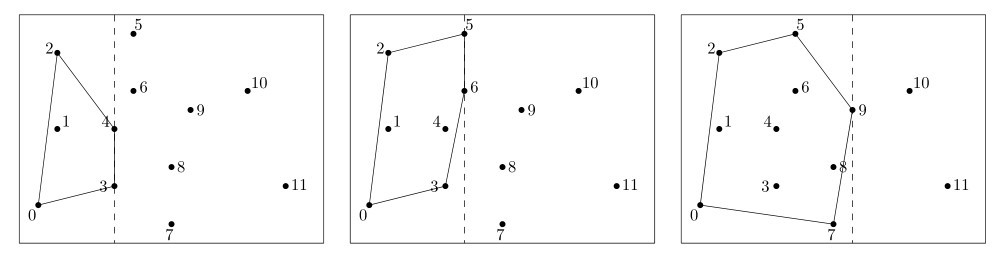
\includegraphics[width=0.9\textwidth]{dm1/figure4.jpg}
    \caption{Diverses étapes dans la procédure de balayage. La droite de balayage est en tirets.}
    \label{fig:fig4}
\end{figure}

\subsection*{D - Algorithme de balayage} Cet algorithme a été proposé par R. Graham en 1972. Nous allons écrire la variante (plus simple) proposée par A. Andrew quelques années plus tard.\\

La première étape consiste à trier les $n$ points du nuage $P$ par ordre croissant d’abscisse, en conservant tous les points de même abscisse dans un ordre arbitraire.\\

À partir de maintenant, on supposera que les points fournis en entrée sont triés par abscisse croissante, comme c’est le cas dans l’exemple du tableau \verb|tab| donné au début du sujet.\\

L’idée de l’algorithme est de balayer le nuage de points horizontalement de gauche à droite par une droite verticale, tout en mettant à jour l’enveloppe convexe des points de $P$ situés à gauche de cette droite, comme illustré dans la figure \ref{fig:fig4}.\\

Plus précisément, l’algorithme visite chaque point de $P$ une fois, par ordre croissant d’abscisse (donc par ordre croissant d’indice de colonne dans le tableau \verb|tab| car celui-ci est trié). À chaque nouveau point $p_i$ visité, il met à jour le bord de l’enveloppe convexe du sous-nuage $\{p_0, \dots , p_i\}$ situé à gauche de $p_i$. On
remarque que les points $p_0$ et $p_i$ sont sur ce bord, et on appelle enveloppe supérieure la partie du bord de $Conv\{p_0, \dots , p_i\}$ située au-dessus de la droite passant par $p_0$ et $p_i$ ($p_0$ et $p_i$ compris), et enveloppe inférieure la partie du bord de $Conv\{p_0, \dots , p_i\}$ située au-dessous ($p_0$ et $p_i$ compris). Le bord de $Conv\{p_0, \dots , p_i\}$
est donc constitué de l’union de ces deux enveloppes, après suppression des doublons de $p_0$ et $p_i$.\\

Par exemple, dans le cas du nuage $P$ de la figure \ref{fig:fig4} gauche, le sous-nuage $\{p_0, p_1, p_2, p_3, p_4\}$ a pour enveloppe supérieure la séquence $(p_0, p_2, p_4)$ et pour enveloppe inférieure la séquence $(p_0, p_3, p_4)$, le bord de son enveloppe convexe étant donné par la séquence $(p_0, p_3, p_4, p_2)$.\\

Informatiquement, les indices des sommets des enveloppes inférieure et supérieure seront stockés dans deux piles d’entiers séparées, $ei$ (pour enveloppe inférieure) et $es$ (pour enveloppe supérieure).

La mise à jour de l’enveloppe supérieure est illustrée dans la figure \ref{fig:fig5} : tant que le point visité ($p_9$ dans ce cas) et les deux points dont les indices sont situés au sommet de la pile $es$ (dans l’ordre : $p_8$ et $p_5$)
forme une séquence $(p_9, p_8, p_5)$ d’orientation négative (voir la définition 1 pour rappel de l’orientation), on dépile l’indice situé au sommet de $es$ (8 dans ce cas). On poursuit ce processus d’élimination jusqu’à ce que l’orientation devienne positive ou qu’il ne reste plus qu’un seul indice dans la pile. L’indice du point visité ($p_9$ dans ce cas) est alors inséré au sommet de $es$. La mise à jour de l’enveloppe inférieure s’opère de manière symétrique.

\begin{figure}[!ht]
    \centering
    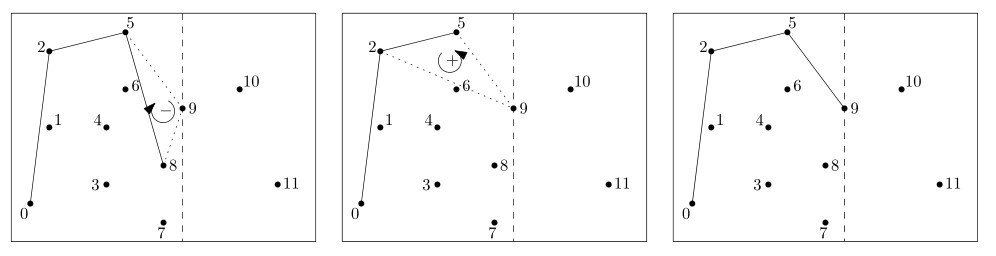
\includegraphics[width=0.9\textwidth]{dm1/figure5.jpg}
    \caption{ Mise à jour de l’enveloppe supérieure lors de la visite du point $p_9$}
    \label{fig:fig5}
\end{figure}

\begin{enumerate}[resume]
\setcounter{enumi}{9}
\item Écrire une fonction \verb|void maj_es(point *tab, stack es, int i);| qui prend en paramètre le tableau  \verb|tab| ainsi que la pile  \verb|es|, non vide, et l’indice  \verb|i| du point à visiter, et qui met à jour l’enveloppe supérieure du sous-nuage. Le temps d’exécution de votre fonction doit être majoré par une constante fois \verb|i|.

\begin{code}{c}{main.c}
void maj_es(point *tab, stack es, int i) {
    int a, b;
    do {
        a = pop(es);
        if (!is_empty(es)) b = top(es);
    } while(orient(tab, i, a, b) < 0);
    
    push(a, es);
    push(i, es);
}
\end{code}

\item Écrire une fonction \verb|void maj_ei(point *tab, stack ei, int i);| qui effectue la mise
à jour de l’enveloppe inférieure, avec le même temps d’exécution.

\begin{code}{c}{main.c}
void maj_ei(point *tab, stack ei, int i) {
    int a, b;
    do {
        a = pop(ei);
        if (!is_empty(ei)) b = top(ei);
    } while (orient(tab, i, a, b) > 0);
    push(a, ei);
    push(i, ei);
}
\end{code}


\item Écrire maintenant une fonction \verb|stack conv_graham(point *tab, int n);| qui prend en
paramètre le tableau \verb|tab| de taille \verb|n| représentant le nuage $P$, et qui effectue le balayage des points de $P$ comme décrit précédemment. On supposera le tableau \verb|tab| déjà trié par ordre croissant d’abscisse.
La pile renvoyée devra contenir les indices des sommets du bord de $Conv(P)$ triés dans l’ordre positif d’orientation, à commencer par le point $p_0$.
Par exemple, sur le nuage de la figure \ref{fig:fig1}, le résultat de la fonction \verb|stack conv_graham| doit être la pile \verb|env| contenant la suite d’indices 0, 7, 11, 10, 5, 2 dans cet ordre, l’indice 0 se trouvant au fond de la pile \verb|env| et l’indice 2 au sommet de \verb|env|.

\begin{code}{c}{main.c}
stack conv_graham(point *tab, int n) {
    stack es = new_stack(), ei = new_stack();
    push(0, es);
    push(1, es);
    push(0, ei);
    push(1, ei);
    for (int k = 2; k < n; k++) {
        maj_es(tabv, es, k);
        maj_ei(tabv, ei, k);
    }
    if (top(es) == top(ei)) pop(es);
    while (top(es) != 0) push(pop(es), ei);
    return ei;
}
\end{code}

\item Analyser brièvement le temps d’exécution de l’algorithme de balayage décrit précédemment, en supposant une fois encore que les points du nuage fourni en entrée sont déjà triés par abscisse croissante. En déduire que le temps d’exécution total de l’algorithme de Graham-Andrew est bien majoré par une constante fois $n \log n$.

\boxans{
    L'algorithme de balayage consiste essentiellement en le calcul de l'enveloppe supérieure et inférieure, deux algorithmes symétriques et donc de même coût temporel. On peut donc s'intéresser au coût temporel du calcul de l'enveloppe supérieure, soit le calcul de la pile $\texttt{es}$.\\
    
    La seule opportunité pour un point $p \in P$ d'indice $i$ d'être ajouté à la pile $\texttt{es}$, puisque l'instruction $\texttt{maj\_es(tabv, es, k = i);}$ n'est appelée qu'une fois avec $k = i$ (dans la boucle $\texttt{for}$ de la fonction $\texttt{conv\_graham}$) et que la fonction $\texttt{maj\_es(point *tab, stack es, int i);}$ ne fait qu'une seule fois appel à l'instruction $\texttt{push(i, es)}$. Tout point $p \in P$ ne peut donc être sorti qu'une seule fois de $\texttt{es}$.\\
    
    Or à chaque itération de la boucle $\texttt{while}$ de la fonction $\texttt{maj\_es}$ correspond une instruction $\texttt{pop(es)}$, soit la sortie d'un point de $\texttt{es}$.
    Sur le calcul de l'enveloppe supérieur d'un nuage $P$, la boucle $\texttt{while}$ de la fonction $\texttt{maj\_es}$ ne pourra donc pas s'exécuter plus de $n = \#P$ fois.
    
    Ainsi \boxsol{le coût temporel du balayage, soit de la fonction $\texttt{conv\_graham}$, est $O(n)$.}\\
    
    Tout algorithme de tri ayant au mieux une complexité en temps linéarithmique $O(n \log n)$, le coût temporel des points du nuage par abscisse croissante est supérieur à celui du balayage. Avec un algorithme de tri optimal, \boxsol{le coût temporel de l'algorithme de Graham-Andrew est $O(n \log n)$}. 
    
}

\end{enumerate}
\end{document}